\section{\uppercase{Code generation pattern}}
\label{sec:codegen}
%\subsection{Transformation pattern}
%todo: describe the pattern

%Transformation from State machine to fUML (classes, attributes, methods)
%\lipsum[1]
This section describes our code generation pattern for states, regions, events, and transitions.

%\subsection{Assumption}
%todo: give some assumptions on code generation such as functions to create methods, attriutes, classes
Assuming that we want to generate from the state machine to an object oriented programming language $ActLang$, which is a C++-like and supports multi-threading by following functions and resource control as mutexes.
\begin{itemize}
	%\item $genClass(n, generals, itfs)$ creates a class with its name, parent class set, and implemented interfaces as \ti{n}, \ti{generals}, and \ti{itfs}.
	
	%\item $genMtd(n, c, type, params)$ creates a method $m$ with its name as $n$ inside the class $c$, its return type as $type$, and $params$ as its parameter set.
	
	%\item $genAttr(n, c, type, multiplicity)$ creates an attribute named $n$ in the class $c$ and typed by $type$. The create attribute is an array if $multiplicity > 1$, otherwise a simple attribute.
	
	%\item $genEnum(n)$ and $genEnumLit(enum, n)$ create an enumeration and its enumeration literal, respectively.
	
	%\item $genBody(m, body)$ adds a body to a method. The body is a string which contains a list of statements.
	
	%\item $createParalle(t, seg)$ generates a mechanism which allows the segment code $seg$ run in a thread $t$. Similarly, $genWait(t), genJoin(t)$.
	
	\item A mutex has three methods $lock$, $unlock$, and $wait$, which automatically unlocks the mutex and waits until it receives a signal.  
	
	%\item $synchronize(seg)$ generates a mechanism which allows the segment code $seg$ run safely (can be either based on \ti{POSIX pthread} or \ti{Java synchronize} mechanism).
	
	%\item $toString(stts)$ is used to convert a list of statements $stts$ into a readable string which can be add to a method as its body.
	
	%\item Concatenation of two strings $str1$ and $str2$ is concisely described as $str1 + str2$.
	
	%\item \ti{WHILE}, \ti{FOR} \ti{IF}, \ti{ELSE} are symbols representing while and for loops, if and else statements.
	
	\item \ti{FORK(func)} creates a thread (lightweight process) associated with the function/method \ti{func} and \ti{JOIN(theThread)} waits until the method associated with the thread \ti{theThread} completes.
\end{itemize} 


\subsection{State}
%Suppose that we want to generate a state machine $sm$ whose states are listed by $lstates$. 
%A common state interface $IState$ is created. The interface contains three methods, namely, \ti{entry}, \ti{exit}, and \ti{doActivity} respectively corresponding to three state actions. The benefice of using these methods is to increase performance in invoking state actions. To preserve the hierarchy of composite states, the interface also has two attributes called \ti{actives} and \ti{pres} referring to current and previous active sub-states in case of the presence of history states.

A common state type $IState$ is created. 
The type 
%three methods, namely, \ti{entry}, \ti{exit}, and \ti{doActivity} respectively corresponding to three state actions. The benefice of using these methods is to increase performance in invoking state actions. To preserve the hierarchy of composite states, the interface also 
has two attributes called \ti{actives}, to preserve the hierarchy of composite states, and \ti{previousActives} referring to current and previous active sub-states in case of the presence of history states.
Each UML state is transformed into an instance of \tb{IState} and a state ID is assigned (which is a child element of an enumeration). 
During initialization, each instance initializes its attributes to a default value meaning inactive state. 

In the following sections, 
we only consider C++ as a specific generated language. 
The discussion of other object-oriented languages is much similar since these share the same concepts.

Listing \ref{lst:IStateCpp} shows the state type and its instances. 
\ti{STATE\_MAX} is the number of states. 
The state actions such as entry/exit/doActivity are generated to corresponding common methods containing action codes.
For example, \ttt{entry} in the listing implements all of the state action codes.
%The actions are named depending on the name of the corresponding. 

%//discuss the limitation of doActivity implementation vs specification.

\begin{lstlisting}[caption=IState interface and function pointers in C++, label=lst:IStateCpp, language=C++,float]
typedef struct IState {
  int previousActives[2];  int actives[2];
} IState;
class C {
private:
  IState states[STATE_MAX];
public:
  void entry(StateId id) {
	  switch{id} {
		  case S0_ID:
			  //action code for each state
			  break;
		  //code for other state actions  
	  }
  }
}
\end{lstlisting}

\begin{comment}
\begin{lstlisting}[mathescape=true, caption=IState interface and annonymous sub-classes in Java, label=lst:IStateJava, frame=single, language=JAVA]
public interface IState {
  public IState[] pres; 
  public IState[] actives;
  public EventId defEvents;
  public void entry();
  public void exit();
  public void doActivity();
}
class C {
private IState states[NUM_STATES];
public C() {
  states[S0_ID] = new IState() {
    public void entry() {
      S0_entry();
    }
    ...
  }
}
public void S0_entry() {...}
}
\end{lstlisting}
\end{comment}

\begin{comment}
The procedure to generate the code for states is shown in Listing \ref{lst:procedure1}. It first creates the state interface $IState$ (in C++, it is either a class or a struct). The array attribute is then created with the number of states as its size. Each state is also associated with a state ID which is a child of an enumeration. Finally, the constructor of $C$ is created to initialize and make methods of the attribute instances refer to \ti{entry/exit/doActivity} action methods of $C$. The implementation of action methods in the context class $C$ is similar to the delegation pattern proposed by the authors in \cite{Niaz2004} but dramatically decreases the memory consumption since only one common interface for all states is created instead of a class for each state in \cite{Niaz2004}.

\begin{lstlisting}[mathescape=true, caption=Procedure to create code for states, label=lst:procedure1, frame=single]
IState = genClass('IState', $\emptyset$, $\emptyset$);
stateIdEnum = genEnum('StateIdEnum');
foreach s in lstates
  genEnumLit(stateIdEnum, s.name + '_ID');
  mtd = genMtd(s.name + '_entry', C, 
			null, null);
  genBody(mtd, toString(entry(s)));
  ...
genEnumLit(stateIdEnum, 'NUM_STATES');  
genAttr('states', C, IState, NUM_STATES); 
genMtd(C.name, C, null, null);
\end{lstlisting}
\end{comment}


State \ttt{doActivity}s, as specified by UML, are run concurrently. 
Each \ti{doActivity} is then run within a permanent thread and a mutex is created for controlling it. 
%The \ti{doActivity} thread is initialized, waits for a start signal, executes the \ti{doActivity} code, generates a completion if the state is atomic and still active, and goes back to the waiting point as the paradigm above. 
Listing \ref{lst:doActivity} shows a code segment for \ti{doActivity} threads. The method \ttt{doActivityThread} takes as input a state id to use and call the appropriate mutex and \ti{doActivity}, respectively. 
The method does nothing and stays in a waiting point if the state corresponding to the input parameter state identifier is inactive (line 5).
If the state is active, a start signal is sent to this thread method to start the execution of \ti{doActivity}.
The generated code typically follows the common paradigm in POSIX threads \cite{Posix}.

\begin{lstlisting}[caption=Example code generated for doActivity, label=lst:doActivity, language=C++,float][H]
while(true) {
	pthread_mutex_lock(&mutex[stateId]);
	while(!isStarts[stateId]) { 
		//await start signal     
		pthread_cond_wait(&cond, &mutex[stateId];}	
	doActivity(stateId);
	isStarts[stateId] = false;//reset wait flag
	pthread_mutex_unlock(&mutex[stateId]);
	if (!isStops[stateId]) {
		if(stateId==S0_ID||...){//atomic states
			pushCompletionEvent(stateId);
		}
	}
}
\end{lstlisting}


\subsection{Region}
\label{subsubsec:region-trans}
Our approach considers regions as elements to be transformed. 
Specifically, each region has two methods: entering and exiting. 
The entering method controls how a region $r$ is entered from an outside transition and the exiting method exits completely a region by executing exit actions of sub-states from innermost to outermost.

\begin{figure}
	\hspace*{-1.2cm}  
	\centering
	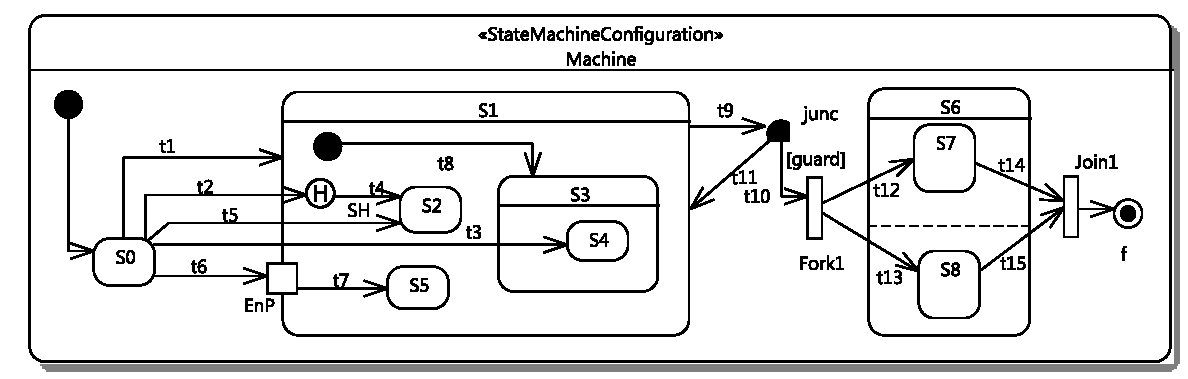
\includegraphics[clip, trim=0.2cm 0.2cm 0.2cm 0.2cm, width=1.0\columnwidth + 1.2cm]{figures/EnteringStateExample.pdf}
	\caption{Example illustrating different ways entering a composite state} 
	\label{fig:entering}
\end{figure}

A region can be entered two different ways: (1) \tb{entering by default}: the transition ends at the border of composite states; and (2) \tb{cross transition}: entering at a direct or an indirect sub-vertex of composite states.
The two entering ways execute the entry action of the containing composite state after the transition effect. 
%\ti{doActivity(ctner(r))} is then signaled to be run in its associated thread. 
The executions afterwards are different for each way. 
To illustrate, we use an example as in Fig. \ref{fig:entering} with \ti{S1} as a target composite state. 
\ti{t1} is in the way (1) while \ti{t2, t5, t6} in the way 2. 

The entering method associated with the region of \ti{S1} has a parameter $enter\_mode$ telling how the entering should be executed. 
$enter\_mode$ takes values depending the number of transitions coming to the composite state. %$S1$: $\#values(s) = \\ \#\{v \in vertices(s)| v.kind=initial\} + \\ \#\{v \in vertices(s)| \exists t \in T_{ins}(v), src(t) \notin vertices(s)\} + \\ 
%\#\{v \in vertices^+(s)\setminus vertices(s)|\exists t \in T_{ins}(v), src(t) \notin vertices^+(s)\}$. 
%In this case these values are $\{DEFAULT = 0, SH\_MODE = 1, S2\_MODE = 2, S4\_MODE=3, ENP_MODE=4\}$. 
The detail of how these modes are implemented in specific languages are not discussed here.
Listing \ref{lst:region} shows the generated C++.

  
\begin{lstlisting}[caption=Example code generated for the region of S1, label=lst:region,float]
void S1Region1Enter(int enter_mode){
if (enter_mode == DEFAULT) {
  states[S1_ID].actives[0] = S3_ID;
  entry(S3_ID);  sendStartSignal(S3_ID);
  S3Region1Enter(DEFAULT);
} else if (enter_mode == S2_MODE) { 
  //..
} if (enter_mode == SH_MODE) {
  StateIDEnum his;
  if (states[S1_ID].previousActives[0]!=STATE_MAX){
    his=states[S1_ID].previousActives[0];
  } else {
    his = S2_ID;
  }
  states[S1_ID].actives[0] = his;
  entry(his);  sendStartSignal(his);
  if (S3_ID == his) {
    S3Region1Enter(S3_REGION1_DEFAULT);
  } 
} else if (enter_mode == S4_MODE) {
  states[S1_ID].actives[0] = S3_ID;
  entry(S3_ID);  sendStartSignal(S3_ID);
  S3Region1Enter(S4_MODE);
} else if (enter_mode == ENP_MODE) {...}
\end{lstlisting}




%For each value in $values(s)$, the region of $S1$ is entered and executes different actions. 
By default, the region's active sub-state is set after the execution of any effect associated with the initial transition. 
Therefore, $S3$ is set as active sub-state of $S1$. 
Entering at (\ti{S2}) sets the active sub-state of \ti{S1} directly to \ti{S2}. 
In case of an indirect sub-state ($S4$), the entry action of $S3$ is executed before $S4$ is set as the active-sub state of $S3$ and the entry execution of $S4$. 
It is worth noting that after the execution of each entry action, a start signal is sent to activate the waiting thread associated with \ti{doActivity} of the corresponding state.

Transitioning from a vertex to a sub-vertex of the composite state (transition from $S0$ to $SH$ is a particular case) is not as simple as that of two states. This is detailed in the next section.


The method generated for exiting a region is simpler than that of entering.
It basically executes the exit actions of all the active sub-states from innermost to outermost.
\subsection{Event}
\label{subsec:event}
Similar to the approach in \cite{niaz_mapping_2004}, one method is generated for each event. 
An event enumeration \ti{EventId} is created whose children are event identifiers associated with events. 
%Suppose $levents$ is the list of events which can be processed by the state machine $sm$. 
The event list of a state machine contains explicitly defined events and a special event called completion event, which is implicitly implemented. 
A completion event is fired when either the execution of the \ti{doActivity} of simple/atomic state completes or all regions of a composite state have reached final states. 
For each event type, the pattern is realized as followings:

\vskip 0.1cm	
\noindent
\tb{CallEvent}:                                            When its associated operation is called, the event processing waits and locks the main mutex protecting the run-to-completion semantics as previously mentioned, and executes the event processing (see \ref{subsec:deadlock}). 

\vskip 0.1cm	
\noindent		
\tb{SignalEvent}:                                          An API \ti{sendSignal} is created for environment code to interact and send an instance of the signal associated with the event by calling it. 
When the API is called, an event is emitted and written into the event queue.                                             
		
		
\vskip 0.1cm	
\noindent		
\tb{TimeEvent}:                                            A thread associated with the event is created and initialized at the initialization.
Within the thread execution, its associated method waits for a signal, which is sent after the execution of the entry of an accepting state, to start sleeping for a duration specified by the event. 
%The state must have at least one outgoing transitions triggered by the event. 
When the relative time expires, the event is emitted and written to the event queue if the state is still active.                                         

\vskip 0.1cm
\noindent		
\tb{ChangeEvent}:                                          Similarly to time events, a thread is initialized and its method waits for a starting signal. 
The method checks whether the value of the boolean expression of the event is updated from false to true. 
If so, the event is committed to the event queue.   
The expression is expressed by attributes of the class owning the state machine.
The starting signal is sent if one of the expression's constituents (attributes of the class) changes.
We track the changes of the attributes' values by using setters of the attributes.
For example, for an expression $x + y > 10$, \ti{x} and \ti{y} are extracted as constituents.
The setters (\ti{setX} and \ti{setY}) are automatically generated.
They do not only affect the value of \ti{x} and \ti{y} but also send the starting signal to the thread.                         


\begin{comment}
\begin{itemize}
	\item \ti{CallEvent} $ce$: The associated operation $op(ce)$ can be either synchronous or asynchronous. When $op(ce)$ is called, it waits and locks the main mutex protecting the run-to-completion semantics, and executes $mtd_{ce}$. Contrarily, the parameters of the asynchronous operation are used to create a signal which is transformed similarly to the case of $SignalEvent$.
	
	\item \ti{SignalEvent} $se$: $SignalEvent$ is asynchronous. 
	The signal associated with $se$ is written into the event queue of the active class $C$ by an operation which takes as input the signal. 
	
	\item \ti{TimeEvent} $te$: A thread $teThread$ associated with $te$ is created and initialized at the initialization of the state machine. 
	Within the execution of $teThread$, the method associated $te$ waits for a signal, which is sent after the execution of the entry of a state $s \in \{v \in V|\exists t \in T_{outs}(v), te \in events(t)\}$, to start sleeping for a duration $d$ of $te$. 
	When the duration expires, $te$ is emitted and written to the event queue if $s$ is still active.
	
	\item \ti{ChangeEvent} $che$: Similar to $TimeEvent$, a thread $cheThread$ is initialized at initialization but the associated method $mtd$ does not wait for a signal to start. $mtd$ periodically checks whether the value of the associated boolean expression $ex(che)$ changes by comparing the current value with the previous value. 
	If a change happen, $che$ is committed to the event queue.
	
	\item \ti{Any}: any of the above events can trigger the associated transitions.
\end{itemize}
\end{comment}

As above presented, all asynchronous incoming events are stored in a runtime priority queue, in which each event type has a priority. Completion event always has the highest priority. 
Others are equal by default. 
%Fig. \ref{fig:eventqueue} shows the generic structure of events stored in the queue.  
Event type, priority, identifier, associated state \ti{stateId} of completion events, and signal data are specified in an internal structure. 
The associated state is responsible to specify which atomic/simple state completes its \ti{doActivity} execution or the composite state whose sub-states have reached final states. 
%The event method associated with \ti{Completion Event} executes a check on \ti{stateId} (see Listing \ref{lst:event}, line 1).
%The event data contain marshaled%\footnote{https://en.wikipedia.org/wiki/Marshalling$\_$(computer$\_$science)} 
%parameters of \ti{SignalEvent}'s signal or \ti{CallEvent}'s parameters.

%\begin{figure}
%	\centering
%	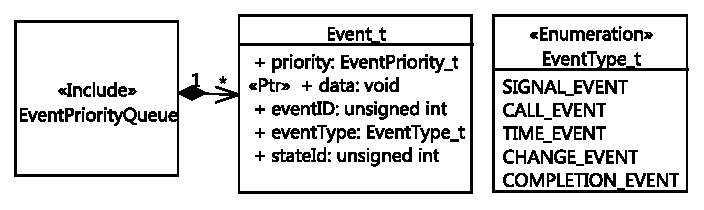
\includegraphics[clip, trim=0.2cm 0.2cm 0.2cm 0.2cm, width=\columnwidth]{figures/eventqueue.pdf}
%	\caption{Event data structure} 
%	\label{fig:eventqueue}
%\end{figure}

\subsection{Transitions}

%To process events, for each event, a method is implemented in $C$. 
Each event triggers a list of transitions. 
%We define $dp(v)$ as a function returning the depth of a vertex $v$, in which $dp(v) = 1$ if $v$ is a top vertex.
We suppose $T_{trig}(e)$ is the transition list triggered by the event $e$, and $S_{trig}(e)$ is a depth-ordered (from innermost to outermost) set of the source states of the transitions in $T_{trig}(e)$. 
%To present how the body of event methods is generated, we define functions as followings:

\begin{comment}
{\small
\begin{itemize}
	\setlength\itemsep{0em}
	\item Vertex depth $dp(v)$ returns the depth of a vertex.
	If $v$ is a top vertex, $dp(v) = 1$.
			%\begin{equation}
			%dp(v) =    \left\{
			%\begin{array}{ll}
			%1 & \ti{v is a root vertex}  \\
			%dp(ctner(v)) + 1& otherwise \\
			%\end{array} 
			%\right.
			%\end{equation}
			
	\item $Map_{e}(s) \subset S_{trig(e)} | \forall sub \in Map_e(s): ctner(sub) = s$.
	%, $Prt(e) = \{s \in V| Map_{e}(v) \neq \emptyset\}$. 
	$Prt(e)$ is an ordered list whose length is $len(Prt\{e\})$ and elements are accessed by indexes. 
	The order of $Prt(e)$ is defined as: $\forall i, j \leq len(Prt\{e\})$, 
	\\ if $i < j, dp(Prt(e).get(i)) \geq dp(Prt(e).get(j))$. 	
\end{itemize}
}
\end{comment}

Algorithm \ref{alg:eventproc} describes how to generate the body of an event method. 
It first finds the innermost active states which are able to react $e$ by orderly looping over $S_{trig}(e)$.
This is to ensure that, in case of multiple transitions triggered by the event, the generated code for the transitions outgoing from innermost states will be executed.    
For each transition from an innermost state, code for active states and deferred events, guard checking, and transition code segments are generated by $GEN\_CHECK$, $GEN\_GUARD(t)$ and \ti{GEN\_TRANS}, respectively. 
If the identifier of $e$ is equal to one of the deferred event list of the corresponding state (not shown in this paper), $GEN\_CHECK$ generates code, which checks whether the event to be deferred and pushes the event to a deferred event queue managed by the runtime main thread.
The latter also pushes the deferred events back to the main queue once one of the pending events is processed and the active state is changed. 

\begin{algorithm}[]
	\linespread{0}
	\caption{Code generation for events
		\label{alg:eventproc}}
	\begin{algorithmic}[1]
		\scriptsize
		\Require{Event $e$}
		\Ensure{Code generation process for event method}
		\Procedure{EventGenProcess}{$e$}
		\For {$\forall$ s $\in S_{trig}(e)$}
			\State {$T_s = \{t \in T_{trig}(e)|src(t) = s\}$}
			\For {$\forall t \in T_s$}
				\State {$GEN\_CHECK(s, t, e)$}
				\State {$GEN\_GUARD(t)$}
				\State {$GEN\_TRANS(s,t,tgt(t))$} 
			\EndFor
		\EndFor			
		\EndProcedure	
	\end{algorithmic}
\end{algorithm}


\begin{comment}
\begin{lstlisting}[mathescape=true, caption=Generation process for an event, label=lst:eventproc, frame=single,float]
$\forall$ item $\in Lm(e)$
  $\forall s \in Map_e(item)$
    $T_s = \{t \in T_{trig}(e)|src(t) = s\}$
    $\forall t \in T_s$
	    $GENERATE\_STATE\_EVENT\_CHECK(s, t, e)$
	    $GENERATE\_GUARD(t)$
      $GENTRANS(s,t,tgt(t))$  	
\end{lstlisting}
\end{comment}



For a transition $t$, $GEN\_CHECK$ can generate single or multiple active state checking code. 
The latter occurs if the target of the transition is a pseudo state join because the transitions incoming to a $join$ are fired if and only if all of their source states are active. 
The detailed discussion on these is not presented due to space limitation. Listing \ref{lst:event}, lines 2-3 show a portion of the code with multiple checking generated for the completion event processing method.
The transitions \ti{t14} and \ti{t15} incoming to $Join1$ are executed if \ti{S6} and \ti{S7} are active. 
In addition, the code portion checks the state associated with the current completion event emitted upon the completion of either \ti{S6}'s or \ti{S7}'s \ti{doActivity}.  
In lines 4-6, the code concurrently exits the sub-states of \ti{S6} by using \ti{FORK} and \ti{JOIN}, which are respectively used to spawn and wait for a thread, for the region methods associated with \ti{S6}'s orthogonal regions, which actually exit \ti{S7} and \ti{S8}. 
Then, \ti{exit(S6)} is executed before the concurrency of transition effects \ti{t14} and \ti{t15} is taken into account.



\begin{lstlisting}[caption=Example code generated for completion events triggering transitions t14 and t15, label=lst:event, language=C++,frame=none,float]
if(event.stateId==S6_ID||event.stateId==S7_ID){
	if (states[S6_ID].actives[0] == S7_ID && 
		states[S6_ID].actives[1] == S8_ID) {
		thread_r1=FORK(S6Region1Exit); 
		thread_r2=FORK(S6Region2Exit);
		JOIN(thread_r1);  	  JOIN(thread_r2);
		sendStopSignal(S6_ID);  exit_S6();
		thread_t14=FORK(effect(t14));  
		thread_t15=FORK(effect(t15));
		JOIN(thread_t14);  JOIN(thread_t15);
		effect_t16();
		activeStateID = STATE_MAX;  //inactive state
	}
}
\end{lstlisting}
  


\begin{algorithm}[]
	\linespread{0}
	\caption{Code generation for transition
		\label{alg:transitiongeneration}}
	\begin{algorithmic}[1]
		\scriptsize
		\Require{A source $v_{s}$, a target vertex $v_{t}$ and a transition $t$}
		\Ensure{Code generation for transition}
		\Procedure{gen\_Trans}{$v_s$, $v_t$, $t$}
%\newline Step 1. Find entry and exit states	
		\State Find $s_{ex}$ and $s_{en}$ as vertexes in the same region and directly or indirectly containing/being $v_{s}$ and $v_{t}$, respectively.
		%\State	$H_s$ = $v_s \cup ctner^+(v_s)$, $H_t$ = $v_t \cup ctner^+(v_t)$
		%\State {$s_{ex} \in H_s, s_{en} \in H_t | ctner(s_{ex}) = ctner(s_{en})$}
		%\Let{\{$s_{ex}, s_{en}$\}}{$FINDEXE(v_s, v_t)$}
		\State Generate IF-ELSE statements for junctions
		\If {$s_{ex}$ is a state}
			\For {$ r \in $ regions of $s_{ex}$}
				\State {$FORK(RegionExit(r))$} //create thread for exiting region
			\EndFor
			\State {Generate JOIN for threads created above}
			\State {Generate sendStopSignal to $s_{ex}$}
			\State {$exit(s_{ex})$} //exit the state	
		\EndIf
		\If {$v_t$ is a pseudo state join}
			\For {$in \in $ incoming transitions of $v_t$}
				\State {$FORK(effect(in))$} //create thread for transition effect
			\EndFor
			\State {Generate JOIN for threads created above}
		\Else 
			\State {$effect(t)$} //execute transition effect
		\EndIf		
		\If {$s_{en}$ is a state}
			\State {$entry(s_{en})$}  //state entry
			\State {Generate sendStartSignal to $s_{en}$}
		\EndIf
		\If {$s_{en}$ is a composite state}
				\For {$ r \in$ regions of $s_{en}$}
				\State {$FORK(RegionEnter(r))$} //create thread for entering region
				\EndFor
			\State {Generate JOIN for threads created above}
		\Else
			\State {Generate for pseudo states by patterns}
		\EndIf
		\EndProcedure	
	\end{algorithmic}
\end{algorithm}



\begin{comment}
Require{A source $v_{s}$, a target vertex $v_{t}$ and a transition $t$} \\
Ensure{Code generation for transition} \\
Procedure{genTrans}{$v_s$, $v_t$, $t$} \\
\step Find entry and exit states \\		
$H_s$ = $v_s \cup ctner^+(v_s)$, $H_t$ = $v_t \cup ctner^+(v_t)$ \\
$s_{ex} \in H_s, s_{en} \in H_t | ctner(s_{ex}) = ctner(s_{en})$ \\
Step 2. Generate IF-ELSE statements for junctions			\\




	\begin{table}[]
		\scriptsize
		\centering
		\caption{Code generation procedure for transition: GENTRANS}
		\label{alg:transitiongeneration}
		\begin{tabular}{p{1cm}p{5.8cm}}
			\hline
			Input & A source $v_{s}$, a target vertex $v_{t}$ and a transition $t$ \\
			Output & Generated code for transition \\
			\hline
			Step 1 & Find entry and exit states \newline
			$H_s$ = $v_s \cup ctner^+(v_s)$, $H_t$ = $v_t \cup ctner^+(v_t)$ \newline $s_{ex} \in H_s, s_{en} \in H_t | ctner(s_{ex}) = ctner(s_{en})$ \\
			Step 2 & Generate IF-ELSE statements for junctions                           \\
			Step 3 & If $s_{ex}$ is a state       \newline
			         \-\hspace{0.2cm} For {$ r \in regions(s_{ex})$}  \newline 
			         \-\hspace{0.4cm} {$FORK(RegionExit(r))$} \newline
			         \-\hspace{0.2cm} {Generate JOIN for threads created above} \newline
			         \-\hspace{0.2cm} {Generate sendStopSignal to $s_{ex}$} \newline   
			         \-\hspace{0.2cm} {$exit(s_{ex})$}    \\
			Step 4 & If $v_t.kind=join$ \newline
					\-\hspace{0.2cm} For {$in \in T_ins(v_t)$} \newline
					\-\hspace{0.4cm} {$FORK(effect(in))$} \newline
					\-\hspace{0.2cm} {Generate JOIN for threads created above}
					                    \\
			Step 5 & If $v_t.kind \not=join$ \newline   
					\-\hspace{0.2cm} {$effect(t)$}                        \\
			Step 6 & If $s_{en}$ is a state \newline
					\-\hspace{0.2cm}   {$entry(s_{en})$} \newline
					\-\hspace{0.2cm}   {Generate sendStartSignal to $s_{en}$}                     \\
			Step 7 & If $s_{en}.kind\in\{conp,conc\}$ \newline
					\-\hspace{0.2cm} For {$ r \in regions(s_{en})$} \newline
					\-\hspace{0.4cm} {$FORK(RegionEnter(r))$}    \newline
					\-\hspace{0.2cm} {Generate JOIN for threads created above}                      \\
			Step 8 & If $s_{en}.kind\notin\{conp,conc\}$ \newline
					\-\hspace{0.2cm}  {Generate for pseudo states by patterns}  \\
			\hline
			                                                 
		\end{tabular}
	\end{table}

\end{comment}

\begin{comment}

\newline Step 3. If $s_{ex}$ is a state
\For {$ r \in regions(s_{ex})$}
\State {$FORK(RegionExit(r))$}
\EndFor
\State {Generate JOIN for threads created above}
\State {Generate sendStopSignal to $s_{ex}$}
\State {$exit(s_{ex})$}	
\newline Step 4. If $v_t.kind=join$
\For {$in \in T_ins(v_t)$}
\State {$FORK(effect(in))$}
\EndFor
\State {Generate JOIN for threads created above}
\newline Step 5. Else
\State {$effect(t)$}	
\newline Step 7. If $s_{en}$ is a state
\State {$entry(s_{en})$}
\State {Generate sendStartSignal to $s_{en}$}
\newline Step 8. If $s_{en}.kind\in\{conp,conc\}$
\For {$ r \in regions(s_{en})$}
\State {$FORK(RegionEnter(r))$}
\EndFor
\State {Generate JOIN for threads created above}
\newline Step 9. Else
\State {Generate for pseudo states by patterns}
\EndProcedure

\begin{algorithm}[]
	\caption{Code generation for transition
		\label{alg:transitiongeneration}}
	\begin{algorithmic}[1]
		\Require{A source $v_{s}$, a target vertex $v_{t}$ and a transition $t$}
		\Ensure{Code generation for transition}
		\Procedure{genTrans}{$v_s$, $v_t$, $t$}
		\Let{$H_s$}{$v_s \cup ctner^+(v_s)$}
		\Let{$H_t$}{$v_t \cup ctner^+(v_t)$}
		\State {$s_{ex} \in H_s, s_{en} \in H_t | ctner(s_{ex}) = ctner(s_{en})$}
		%\Let{\{$s_{ex}, s_{en}$\}}{$FINDEXE(v_s, v_t)$}
		\State {//Generate IF-ELSE statements for junctions}
		\If {$s_{ex}$ is a state}
		\For {$ r \in regions(s_{ex})$}
		\State {$FORK(RegionExit(r))$}
		\EndFor
		\State {//Generate JOIN for threads created above}
		\State {//Generate sendStopSignal to $s_{ex}$}
		\State {$exit(s_{ex})$}	
		\EndIf
		\If {$v_t.kind=join$}
		\For {$in \in T_ins(v_t)$}
		\State {$FORK(effect(in))$}
		\EndFor
		\State {//Generate JOIN for threads created above}
		\Else
		\State {$effect(t)$}	
		\EndIf
		\If {$s_{en}$ is a state}
		\State {$entry(s_{en})$}
		\State {//Generate sendStartSignal to $s_{en}$}
		\If {$s_{en}.kind\in\{conp,conc\}$}
		\For {$ r \in regions(s_{en})$}
		\State {$FORK(RegionEnter(r))$}
		\EndFor
		\State {//Generate JOIN for threads created above}
		\EndIf
		\Else
		\State {//Generate for pseudo states by patterns}
		\EndIf
		\EndProcedure	
	\end{algorithmic}
\end{algorithm}
\end{comment}

 
 

%It generates the code checking for active states respecting the UML semantics in which the innermost states process the incoming event first. To do this, it first looks in the source state list $S_{trig(e)}$ for the innermost states that accept the event triggering its outgoing transitions. If these found states are children of a concurrent state, $genStateCheck$ generates the checking codes run in parallel, which will be described later in \ref{subsubsec:thread}. Otherwise said, sequential code is generated.


\begin{comment}



\begin{algorithm}[]
	\caption{Find states should be exited and entered
		\label{alg:findexit-entry}}
	\begin{algorithmic}[1]
		\Require{A source $v_{s}$ and a target vertex $v_{t}$}
		\Ensure{Vertexes $s_{ex}$, $s_{en}$ to be exited, and entered, respectively}
		\Procedure{findExE}{$v_s$, $v_t$}
			\Let{$H_s$}{$v_s \cup ctner^+(v_s)$}
			\Let{$H_t$}{$v_t \cup ctner^+(v_t)$}
			\State {$s_{ex} \in H_s, s_{en} \in H_t | ctner(s_{ex}) = ctner(s_{en})$}
		\EndProcedure	
	\end{algorithmic}
\end{algorithm}
\end{comment}

\begin{comment}
\begin{itemize}
	\item $join$: Use $GENTRANS$ for $v$'s outgoing transition.
	
	\item $fork$: Use $FORK$ and $JOIN$ for each of outgoing transitions of $v$.
	
	\item $choice$: For each outgoing, an $IF-ELSE$ is generated for the guard of the outgoing together with code generated by $GENTRANS$ (see Listing \ref{lst:event1}).
	
	\item $junction$: As a static version $choice$, a $junction$ is transformed into an attribute $junc_attr$ and evaluated before any action executed in compound transitions (see Listing \ref{lst:event1}). 
	The value of $junc_attr$ is then used to choose the appropriate transition at the place of $junction$.
	
	\item \ti{shallow history}: The identifiers of states to be exited are kept in $pres$ of $IState$. Restoring the active states using the history is exampled as in Listing \ref{lst:region}. The entering method is executed as default mode at the first time the corresponding composite state is entered (see Listing \ref{lst:region}). \ti{pres} is updated with the active state identifier before exiting the region containing the history.
	
	\item \ti{deep history}: Saving and restoring active states are done at all state hierarchy levels from the composite state containing the deep history down to atomic states. Updating \ti{pres} is committed before exiting the region, which is directly or indirectly contained by a parent state, in which a deep history is present.  
	
	\item $enpoint$: If $enpoint$ has no outgoing transition, the corresponding composite state is entered by default. Otherwise said, $GENTRANS$ is called to generate code for the outgoing transition.
	
	\item $expoint$: The code for the unique transition outgoing from $expoint$ is generated by using $GENTRANS$.
	
	\item $terminate$: The code executes the exit action of the innermost active state, the effect of the transition and destroys the state machine object.
\end{itemize}
\end{comment}







\begin{lstlisting}[caption=Example code generated for $Fork1$ and $junc$, label=lst:event1, language=C++,frame=none,float]
if(activeRootState==S1_ID) {
  junc = 0; //outgoing transition t9 of junc
  if (guard) {junc = 1;}
  //Exit substates of S1 and S1
  effect(t9);
  if(junc==0) {
	  effect(t11);
  } else {
	  effect(t10)
  }
  FORK(effect(t12)); FORK(effect(t3)); 
  //JOIN ... ==> concurrent execution
  //Enter state S6, S7 and S8
}
\end{lstlisting}


\ti{GEN\_TRANS} is able to generate code for transitions between two vertexes. 
Algorithm \ref{alg:transitiongeneration} shows how it works. 
The generated code is contained by the deferral events, active states, and guard checking.

Firstly, Algorithm \ref{alg:transitiongeneration} looks for the $s_{ex}$ and $s_{en}$ vertexes contained in the same region and respectively containing the source and target vertexes of the transition $t$.
For example, $s_{ex}$ and $s_{en}$ in case of the $t3$ transition are $S0$ and $S1$ contained by the top region.
If the transition $t$ is part of a compound transition (we use the algorithm presented in \cite{balser2004interactive,Knapp2004} to compute compound transitions), which involves some $junction$s, IF-ELSE statements for junctions are generated first (as PSSM says $junction$ is evaluated before any action). 
The composite state is exited by calling the associated exiting region methods (FORK and JOIN for orthogonal regions) in lines 4-9 and followed by the generated code of transition effects (lines 10-15). 
If the parent state $s_{en}$ of the target vertex $v_t$ is a state (composite state), the associated entry is executed (lines 16-18).
Entering region methods are then called once the above code completes its execution (lines 19-24). 
If the target $v_t$ of the transition $t$ is a pseudo state, the generation pattern corresponding to the pseudo-state types is called. These patterns are shown in Table \ref{table:pseudo-patterm}.

Note that, the procedure in \ref{alg:transitiongeneration} only applies for external transitions. Due to space limitation, the detail of generating local and internal transitions is not discussed here but the only difference is that the composite state containing the transitions is not exited.


\begin{table}[]
	\scriptsize
	\centering
	\caption{Pseudo state code generation pattern}
	\label{table:pseudo-patterm}
	\begin{tabular}{p{0.5cm}|p{6.8cm}}
		%\hline
		Pseudo state                                               & Code generation pattern                            \\ \hline
		join                                                       & Use $GEN\_TRANS$ for $v$'s outgoing transition (Listing \ref{lst:event}, lines 4-6). \\ \hline
		fork                                                       &  Use $FORK$ and $JOIN$ for each of outgoing transitions of $v$ (see Listing \ref{lst:event1}, lines 11-12).                                             \\ \hline
		choice                                                     &      For each outgoing, an $IF-ELSE$ is generated for the guard of the outgoing together with code generated by $GEN\_TRANS$.                                         \\ \hline
		junction                                                   &                   As a static version $choice$, a $junction$ is transformed into an attribute $junc_{attr}$ and evaluated before any action executed in compound transitions (see Listing \ref{lst:event1}, lines 2-3 and 6-10). 
		The value of $junc_{attr}$ is then used to choose the appropriate transition at the place of $junction$.                            \\ \hline
		\begin{tabular}[c]{@{}l@{}}shallow \\ history\end{tabular} &                The identifiers of states to be exited are kept in $previousActives$ of $IState$. 
		Restoring the active states using the history is exampled as in Listing \ref{lst:region}. 
		The entering method is executed as default mode at the first time the composite state is entered (lines 9-19). 
		\ti{previousActives} is updated with the active state identifier before exiting the region containing the history.                               \\ \hline
		\begin{tabular}[c]{@{}l@{}}deep \\ history\end{tabular}    &                   Saving and restoring active states are done at all state hierarchy levels from the composite state containing the deep history down to atomic states. 
		Updating \ti{previousActives} is committed before exiting the region, which is directly or indirectly contained by a parent state, in which a \ti{deep history} is present.                            \\ \hline
		entry point                                                &        If an \ti{entry point} has no outgoing transition, the composite state is entered by default. 
		Otherwise said, $GEN\_TRANS$ is called to generate code for each outgoing transition.                                       \\ \hline
		exit point                                                 &          The code for each transition outgoing from an \ti{exit point} is generated by using $GEN\_TRANS$. If the \ti{exit point} has multiple incoming transitions from orthogonal regions, it is generated as a $join$ to multiple-check the source states of these incomings.                                    \\ \hline
		terminate                                                  &                 The code executes the exit action of the innermost active state, the effect of the transition and destroys the state machine object.                              \\ \hline
	\end{tabular}
\end{table}



\begin{comment}
\subsubsection{Example Code} Listing \ref{lst:event} shows a code segment generated for the processing of $verifyingPIN$. Single checking (line 1) checks whether $Idle$ is the current active state, in which $activeStateID$ is the identifier of the current root active state. The $doActivity$ behavior of $Idle$ is then stopped upon receiving a stop signal. The effect of $t2$, $effect(t3)$ and $effect(t4)$ are then executed after $exit(Idle)$. The execution of $emtry(Verifying)$ then follows the changing of root active state to $Verifying$. $doActivity(Verifying)$ is triggered and followed by concurrently entering the two orthogonal regions of $Verifying$ with appropriate modes.

The discussion of Listing \ref{lst:event1} is similar to Listing \ref{lst:event} except that a multiple checking is executed (line 1-2) instead of a single one. The evaluation for $Junction1$ is executed (line 4) before any other actions (semantic conformance) to decide the decision should be taken (line 10-17). 
\end{comment}
 


 

